\setstretch{1.0}
\chapter{From Sensor to Source: Forward and Inverse Solutions}\label{chapter_meg_source}

In this chapter the fundamental principles of source space reconstruction of MEG sensor data are covered briefly. Whilst not exhaustive, this chapter introduces the generative model of the brain, which provides us with a basis for source reconstruction. In addition, the mathematical framework of the forward and inverse solutions is laid out for use in later chapters in this thesis, with particular focus on spatial filtering techniques. Finally, an investigation into whether the choice of inverse solution has a profound effect on the results of an established functional connectivity pipeline is described. 

\doublespacing
\section*{Introduction}
The magnetic fields that form the basis of MEG are measured using $\sim$300 discrete detectors placed  $\sim$2-4cm from the scalp surface. It is possible to undertake functional connectivity analysis in “sensor space” via assessment between signals measured at separate detectors. However, this comes with three distinct disadvantages:

\begin{enumerate}
	\item \textbf{Field Spread:} The spatial extent of magnetic fields around a current dipole means that multiple sensors will detect signals from a single source which could be erronously interpreted as connections between channels (note this analogous to volume conduction in EEG). \citep{Nunez2006,Scoffelen2009}.
	\item \textbf{Signal Superposition:} A single MEG sensor records a complex mixture of signals generated by many sources, making connectivity assessment between sensors difficult to interpret.
	\item \textbf{Interference:} The magnetic fields generated by the brain are smaller than those generated by external environmental interference (e.g. 50/60 Hz mains electricity). In addition, biological interference, for example from a subject's heart, is larger than the neuromagnetic fields of interest. Interference typically affects many MEG sensors, and hence is highly likely to artificially increase functional connectivity when it is calculated as statistical dependency between sensors. 
\end{enumerate}

The limitations with sensor space analysis are well documented \citep{Scoffelen2009}. Whilst highly successful and meaningful connectivity analyses have been undertaken in this way \citep{Stam2004,Bassett2006,Liu2010}, the inference is usually based on a global parameter (i.e. an integrated measure of global connectivity collapsed across all possible sensor pairs). This means that sensor analysis provides only limited means of interpreting precisely which brain regions or networks are involved. The most successful means to ameliorate the confounds of sensor based connectivity analysis is to apply source space modelling \citep{Scoffelen2009}. This essentially involves mathematically reconstructing the timecourses of electrical activity across many locations (voxels \citep{Hipp2012} or parcellated regions \citep{Hillebrand2012,Tewarie2014a}) in the brain prior to assessment of connectivity between signals reconstructed at those locations. Despite the fact that this projection is mathematically ill posed \citep{Hadamard1902}, there now exists verifiable ways by which to achieve accurate spatial localisation of neural sources, through the use of electromagnetic phantoms (typically supplied with MEG systems for calibration checks routine maintenance) it is possible to test the accuracy of many inverse solutions, for reconstruction of distributed sources and potentially for mapping functional connections. 

In this chapter, we review the theory behind the algorithms which attempt to localise neuronal sources in the brain using extracranial sensor data. Section \ref{sec_gen_model} begins by describing mathematically the generative model which these algorithms attempt to solve. Section \ref{sec_forward_problemn} introduces the forward models used to describe the magnetic field patterns seen on sensor arrays. Section \ref{sec_inverse_problem} introduces the algorithms required to project the data back into source space and finally in Section \ref{sec_bf_v_mn} we present experimental work conducted (by the author) to investigate what effect the choice of inverse solution has on functional connectivity analysis. 

\section{A Generative Model of Sources}\label{sec_gen_model}
The brain contains many possible sources of current dipoles. The measured magnetic fields  outside the head, $\mathbf{b}(t)$, an $n$ element column vector where $n$ is the number of sensors in a system, are the superposition of all the fields generated from the dipoles within the brain volume, $V$ such that,

\begin{equation}
\mathbf{b}(t) = \int_V \mathbf{l}_\mathbf{\theta}q_\mathbf{\theta}(t) dV, \label{eqn_gen_model_1}
\end{equation} where $\mathbf{l}_{\mathbf{\theta}}$ are the lead fields, a model of the magnetic fields for a dipole of unit strength for a given position and orientation vector $\mathbf{\theta}$, and $q_{\mathbf{\theta}}$ is the corresponding dipole strength. Note that it is assumed throughout this thesis, that the lead fields for a source are independent of time, and source orientation is assumed to be constant throughout an experiment. If the brain volume is discretised into a series of $M$ voxels and we assume that only one dipole exists per voxel, we can form the summation

\begin{equation}
\mathbf{b}(t) = \sum_{m=1}^M\mathbf{l}_{\mathbf{\theta}_m}q_{\mathbf{\theta}_m}(t),
\label{eqn_gen_model_2}
\end{equation} it is then possible to introduce a set of composite lead field and dipole vectors:

\begin{equation}
	\begin{aligned}
		\mathbf{L}_V &= 
		\begin{bmatrix} 
			\mathbf{l}_{\mathbf{\theta}_1} & \mathbf{l}_{\mathbf{\theta}_2} & \hdots & \mathbf{l}_{\mathbf{\theta}_M}
		\end{bmatrix},\\
		\mathbf{q}_V(t) &= 
		\begin{bmatrix} 
			q_{\mathbf{\theta}_1}(t) \\ q_{\mathbf{\theta}_2}(t) \\ \vdots \\ q_{\mathbf{\theta}_M}(t)
		\end{bmatrix},
	\end{aligned}	
\end{equation} where $\mathbf{L}_V$ is a $n \times M$ (sensors $\times$ voxels) matrix containing all the information on how the dipoles map to all sensors, and for a given point in time $\mathbf{q}_V(y)$ is a $M\times1$ vector with all the instantaneous dipole strengths. The generative model can now be explained in terms of matrices:

\begin{equation}
\mathbf{b}(t) = \mathbf{L}_V\mathbf{q}_V(t). \label{eqn_gen_model_3}
\end{equation} Note that Equations \ref{eqn_gen_model_1}, \ref{eqn_gen_model_2} and \ref{eqn_gen_model_3} are all equivalent to each other, just expressed differently. 

\section{Estimating the Lead Fields: The Forward Problem}\label{sec_forward_problemn}
To determine the lead fields in Equation \ref{eqn_gen_model_3}, the forward problem needs addressing, which asks: \emph{for a known distribution of current dipoles in the brain, can the associated field pattern be determined?}  Because the magnetic permeability of the head is approximately similar to that of free space ($\mu_r=1$) we can simplify the forward models by treating the entire medium as homogeneous. It is therefore possible to model these dipolar patterns if only the geometric properties of the space between the source and sensor are known. This is in contrast to forward modelling in EEG, as the conductive properties of the skull mean that electric potentials are distorted on detection, meaning complex (and computationally expensive) numerical models such as boundary element models (BEMs) are required.

\subsection{Single Sphere Model}

A model to explain the magnetic field patterns from a source in the brain was developed by \cite{Sarvas1987} and is still the basis of many modern source analyses. The model explains what the field pattern outside a conductive volume would look like if the current is modelled as a dipole within. The electromagnetic fields arising from a bioelectric source with current density $\mathbf{J}$ in a volume $G$ with a constant conductivity $\sigma$ bound by a surface $S$, can be modelled with Maxwell's equations:

\begin{equation}
	\begin{aligned}
		\mathbf{\nabla}\cdot\mathbf{E} &= \frac{\rho}{\epsilon}, \\
		\mathbf{\nabla}\cdot\mathbf{B} &= 0, \\
		\mathbf{\nabla}\times\mathbf{E} &= -\frac{\partial\mathbf{B}}{\partial t}, \\
		\mathbf{\nabla}\times\mathbf{B} &= \mu_0\bigg(\mathbf{J}+\frac{\partial\mathbf{E}}{\partial t}\bigg),
	\end{aligned}\label{eqn_sarvas1}
\end{equation} where $\mu$ and $\epsilon$ are the permeability and permittivity of a medium respectively and $\rho$ is the charge density. As the electromagnetic fields from the brain vary in time at low frequencies (typically < 100 Hz), they are said to be quasi-static (\citealp{Hamalainen1993}; $\frac{\partial}{\partial t}X = 0$, where $X$ is a general function). With this considered, Equation \ref{eqn_sarvas1} can be modified:

\begin{figure}
	\begin{center}
		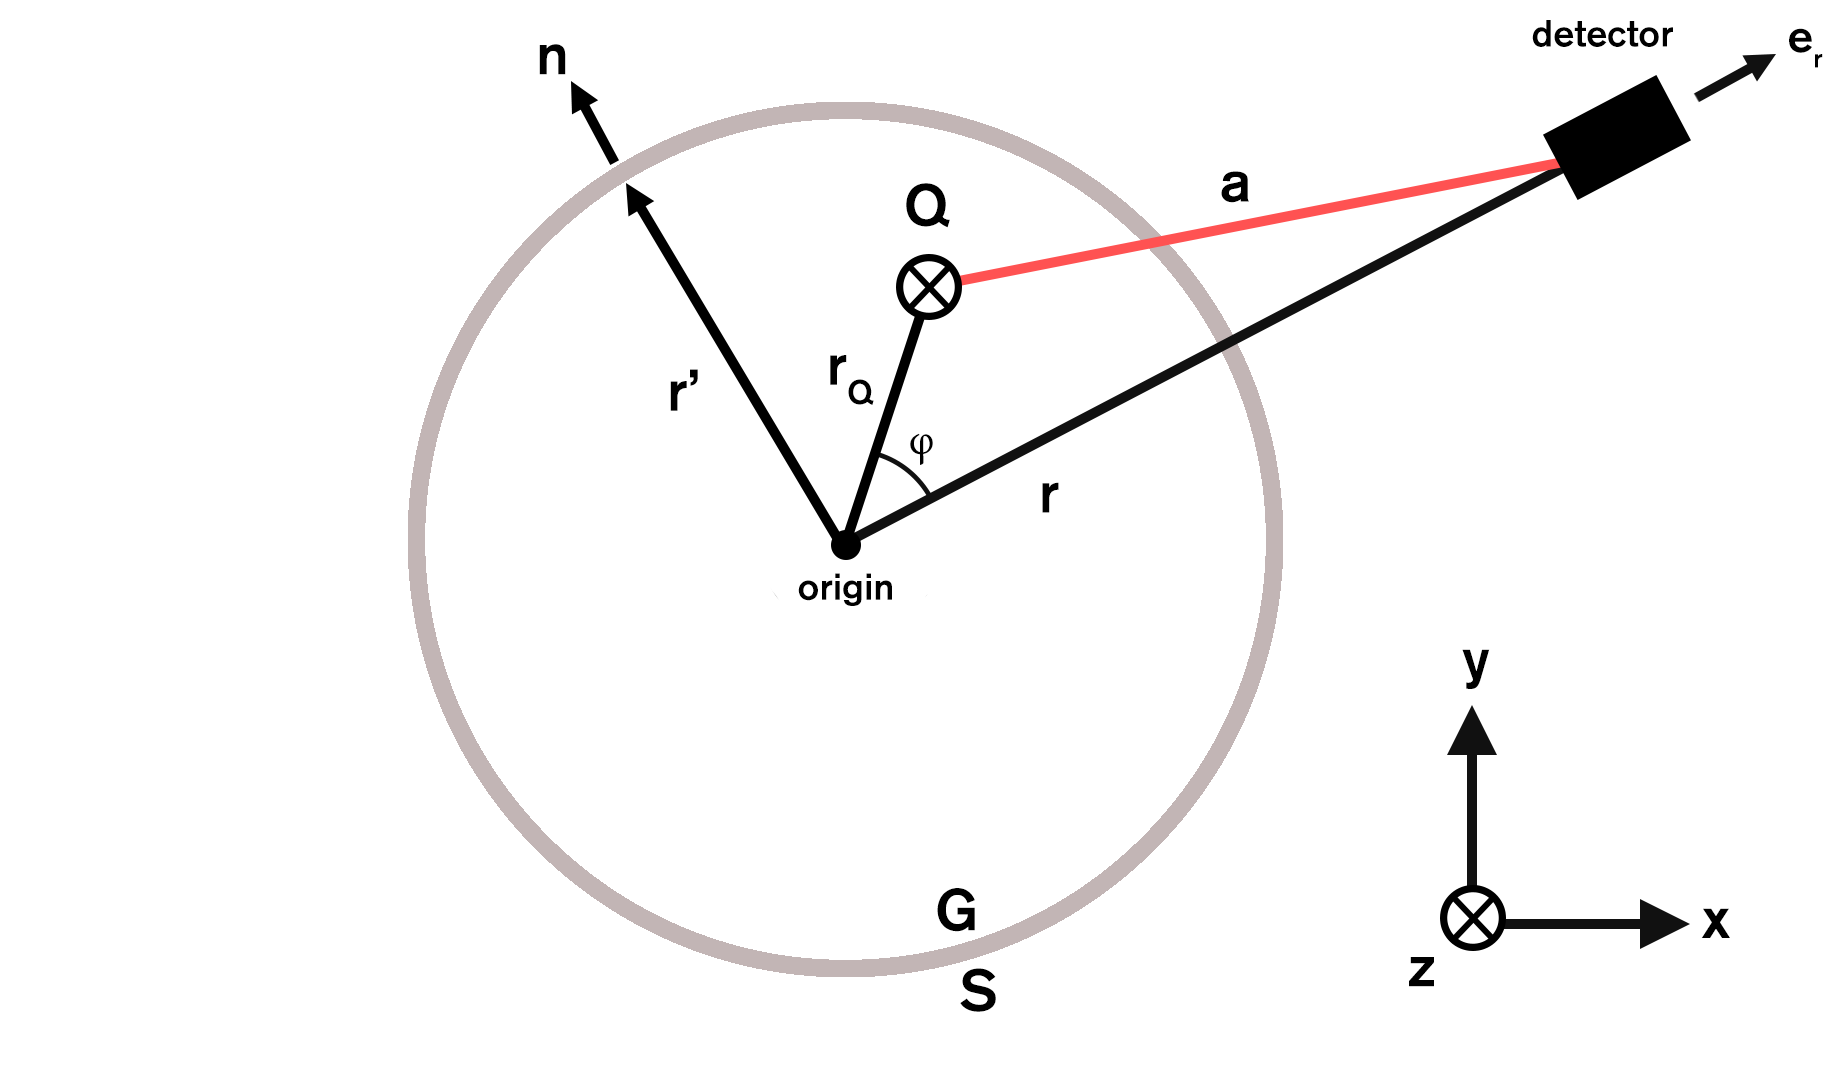
\includegraphics[width=\linewidth]{./images/chapter2/Figure_1.png}
		\caption{An illustration of the single sphere model with a dipole \textbf{Q} at location \textbf{r}\textsubscript{Q}. The spherical volume conductor, G bounded by a spherical surface, S. A detector is placed at location \textbf{r} and we consider the fictitious current (which is non existent, but aids the mathematical analysis) at \textbf{r}'. \label{figure_2_1}}
	\end{center}
\end{figure}

\begin{equation}
	\begin{aligned}
	%\mathbf{E} &= -\mathbf{\nabla}V,\\
	\mathbf{\nabla}\times\mathbf{E} &= 0, \\
	\mathbf{\nabla}\times\mathbf{B} &= \mu_0\mathbf{J}, 
	\end{aligned}\label{eqn_sarvas1a}
\end{equation} Given that $\mathbf{J}$ is the total current density then $\mathbf{B}$ is given by the Ampére-Laplace law:

\begin{equation}
\mathbf{B}(\mathbf{r}) = \frac{\mu_0}{4\pi}\int_{G}\mathbf{J}(\mathbf{r}')\times\frac{\mathbf{r}-\mathbf{r}'}{|\mathbf{r}-\mathbf{r}'|^3}\text{d}\nu', \label{eqn_sarvas2}
\end{equation} where $\mathbf{r}'$ represents a location of a dipole in the volume $G$, $\mathbf{r}$ is a location outside of the volume (as shown in Figure \ref{figure_2_1}) and $\text{d}\nu'$ is a volume element. For a post-synaptic current we can define the current density as

\begin{equation}
\begin{aligned}
\mathbf{J}_\text{PS} &= \mathbf{J}^P+\mathbf{J}^V \\
&= \mathbf{J}^P - \sigma\mathbf{\nabla}V \label{eqn_2_8}
\end{aligned}
\end{equation} where $\mathbf{J}^P$ and $\mathbf{J}^V = - \sigma\mathbf{\nabla}V$ are the primary and volume current densities respectively (see Figure \ref{fig_1_b2}). By defining $\mathbf{R} = \mathbf{r}-\mathbf{r}'$ by substituting Equation \ref{eqn_2_8} into \ref{eqn_sarvas2} we can define $\mathbf{B}$ in terms of the primary and volume currents of a dendrite: 

\begin{equation}
	\begin{aligned}
		\mathbf{B}(\mathbf{r}) &= \frac{\mu_0}{4\pi}\int_{G}\Big(\mathbf{J}^P(\mathbf{r}')-\sigma\mathbf{\nabla}V(\mathbf{r}')\Big)\times\frac{\mathbf{R}}{|\mathbf{R}|^3}\text{d}\nu' \\
		&= \frac{\mu_0}{4\pi}\int_{G}\mathbf{J}^P(\mathbf{r}')\times\frac{\mathbf{R}}{|\mathbf{R}|^3}\text{d}\nu' - \frac{\mu_0\sigma}{4\pi}\int_{G}\mathbf{\nabla}V(\mathbf{r}')\times\frac{\mathbf{R}}{|\mathbf{R}|^3}\text{d}\nu'. \label{eqn_amplaplace}
	\end{aligned}
\end{equation} Here, the first term represents the contribution of the primary current to the magnetic field, and is invariant to conductivity. Briefly, we focus on the term which corresponds to the volume current: 

\begin{equation}
\mathbf{B}^V(\mathbf{r}) = - \frac{\mu_0\sigma}{4\pi}\int_{G}\mathbf{\nabla}V(\mathbf{r}')\times\frac{\mathbf{R}}{|\mathbf{R}|^3}\text{d}\nu',
\label{eqn_volume_magentic_field}
\end{equation}if we recall the vector identity $\mathbf{\nabla}a\times\mathbf{\nabla}b = \mathbf{\nabla}\times(a\mathbf{\nabla}b)$, and assume $\mathbf{\nabla}a=\mathbf{\nabla}V$ and $\mathbf{\nabla}b = \mathbf{R}|\mathbf{R}|^{-3}$, we can rewrite Equation \ref{eqn_volume_magentic_field} so that

\begin{equation}
\mathbf{B}^V(\mathbf{r}) = - \frac{\mu_0\sigma}{4\pi}\int_{G}\mathbf{\nabla}\times V(\mathbf{r}')\frac{\mathbf{R}}{|\mathbf{R}|^3}\text{d}\nu'. \label{eqn_stokes} 
\end{equation} Next, we recall the generalised Stokes theorem 

\begin{equation}
	\int_G\mathbf{\nabla}\times\mathbf{X}\text{d}\nu'=\int_S\mathbf{n}\times\mathbf{X}\text{d}s 
\end{equation} where \textbf{n} is a vector normal to the surface element $\text{d}s$ (directed outwards from the volume centre). Combining Equations \ref{eqn_amplaplace}, \ref{eqn_volume_magentic_field} and \ref{eqn_stokes} we arrive at a new expression for \textbf{B}(r):

\begin{equation}
\begin{aligned}
	\mathbf{B}(\mathbf{r}) &= \frac{\mu_0}{4\pi}\int_{G}\mathbf{J}^P(\mathbf{r}')\times\frac{\mathbf{R}}{|\mathbf{R}|^3}\text{d}\nu' - \frac{\mu_0\sigma}{4\pi}\int_SV(\mathbf{r}')\mathbf{n}(\mathbf{r}')\times\frac{\mathbf{R}}{|\mathbf{R}|^3}\text{d}s \\ 
	&= \mathbf{B}_0(\mathbf{r}) - \frac{\mu_0\sigma}{4\pi}\int_SV(\mathbf{r}')\mathbf{n}(\mathbf{r}')\times\frac{\mathbf{R}}{|\mathbf{R}|^3}\text{d}s,
	\label{eqn_geselowitz}
	\end{aligned}
\end{equation} Equation \ref{eqn_geselowitz} is a modified version of the Geselowitz formula \citep{Geselowitz1970}, which states that the volume current can be represented as a set of fictitious currents (non existent currents which aid the mathematical formulation) flowing on a conductive surface, \textit{S}. Physically, such currents are non existent but otherwise prove useful for further calculations. If we now assume the volume \textit{G} to be bound within a spherical surface \textit{S}, and that the MEG system can only detect the radial component of a magnetic field such that:
\begin{equation}
\begin{aligned}
B_r(\mathbf{r}) &= \mathbf{B}(\mathbf{r})\cdot\mathbf{e}_r \\
& = \frac{\mu_0}{4\pi}\int_{G}\mathbf{J}^P(\mathbf{r}')\times\frac{\mathbf{r}-\mathbf{r}'}{|\mathbf{r}-\mathbf{r}'|^3}\cdot\mathbf{e}_r\text{d}\nu' - \frac{\mu_0\sigma}{4\pi}\int_SV(\mathbf{r}')\mathbf{n}(\mathbf{r}')\times\frac{\mathbf{r}-\mathbf{r}'}{|\mathbf{r}-\mathbf{r}'|^3}\cdot\mathbf{e}_r\text{d}s
\end{aligned}
\end{equation} where $\mathbf{e}_r$ is the unit vector normal to the plane of a MEG sensor. Focussing on a term in the surface integral:

\begin{equation}
\begin{aligned}
 \mathbf{n}(\mathbf{r}')\times(\mathbf{r}-\mathbf{r}')\cdot\mathbf{e}_r &= \Big(\mathbf{n}(\mathbf{r}')\times\mathbf{r}-\underset{\parallel}{\underbrace{\mathbf{n}(\mathbf{r}')\times\mathbf{r}'}}\Big)\cdot\mathbf{e}_r \\
 &=\underset{\perp}{\underbrace{\mathbf{n}(\mathbf{r}')\times\mathbf{r}\cdot\mathbf{e}_r}} \\
 &=0
 \end{aligned} 
\end{equation} means that the surface integral term vanishes, leaving an expression for $B_r$ which is not dependent on the volume currents and crucially, invariant to conductivity:

\begin{equation}
	\begin{aligned}
		B_r(\mathbf{r}) &= \frac{\mu_0}{4\pi}\int_{G}\mathbf{J}^P(\mathbf{r}')\times\frac{\mathbf{r}-\mathbf{r}'}{|\mathbf{r}-\mathbf{r}'|^3}\cdot\mathbf{e}_r\text{d}\nu'. \\
		&= \mathbf{B}_0(\mathbf{r})\cdot\mathbf{e}_r
		\label{eqn_Br_no_conduction}
	 \end{aligned}
\end{equation} Now, we introduce the idea that current from a dipole is not equally distributed across the volume, but rather exists at a single point in space (\textbf{r}\textsubscript{Q}) as a current dipole, 

\begin{equation}
\mathbf{J}^P(\mathbf{r}') = \mathbf{Q}\delta(\mathbf{r}'-\mathbf{r}_Q),
\end{equation} where \textbf{Q} represents the magnitude and direction of the dipole and $\delta$ is the Dirac delta function. Using this allows us to simplify the integral in Equation \ref{eqn_Br_no_conduction}

\begin{equation}
\begin{aligned}
B_r(\mathbf{r}) &= \frac{\mu_0}{4\pi}\int_{G}\mathbf{Q}\delta(\mathbf{r}'-\mathbf{r}_Q)\times\frac{\mathbf{r}-\mathbf{r}'}{|\mathbf{r}-\mathbf{r}'|^3}\cdot\mathbf{e}_r\text{d}\nu' \\
&= \frac{\mu_0}{4\pi} \mathbf{Q}(\mathbf{r}_Q)\times\frac{\mathbf{r}-\mathbf{r}_Q}{|\mathbf{r}-\mathbf{r}_Q|^3}\cdot\mathbf{e}_r \\
%&= \frac{\mu_0}{4\pi} \Bigg(\frac{\mathbf{Q}(\mathbf{r}_Q)\times\mathbf{r}\cdot\mathbf{e}_r}{|\mathbf{r}-\mathbf{r}_Q|^3} - \frac{\mathbf{Q}(\mathbf{r}_Q)\times\mathbf{r}_Q\cdot\mathbf{e}_r}{|\mathbf{r}-\mathbf{r}_Q|^3} \Bigg) \\
%&= -\frac{\mu_0}{4\pi}\frac{\mathbf{Q}\times\mathbf{r}_Q\cdot\mathbf{e}_r}{|\mathbf{r}-\mathbf{r}_Q|^3}
\end{aligned}
\end{equation} To calculate the other components of the magnetic field outside the volume, we note that $\mathbf{J}=0$ outside of $G$ and therefore according to Equation \ref{eqn_sarvas1a}, $\mathbf{\nabla}\times\mathbf{B} = 0$, allowing us to express the magnetic field in terms of the magnetic scalar potential, $U$:

\begin{equation}
	\mathbf{B}(\mathbf{r}) = -\mu_0\mathbf{\nabla}U(\mathbf{r}). \label{eqn_pot_formula}
\end{equation} To determine an expression for $U$, we need to fix \textbf{r} to be outside of $G$ and consider a line integral of $\mathbf{\nabla}U$ along the radius of $G$, $0 \leq t \leq \infty$. As $U$ is a vanishing term at infinity, we obtain

\begin{equation}
	\begin{aligned}
		U(\mathbf{r}) &= - \int_0^\infty \mathbf{\nabla}U(\mathbf{r}+t\mathbf{e}_r)\cdot\mathbf{e}_r\text{d}t \\
		&= \frac{1}{\mu_0}\int_0^\infty B_r(\mathbf{r}+t\mathbf{e}_r)\text{d}t \\
		&= \frac{1}{\mu_0}\int_0^\infty \mathbf{B}_0(\mathbf{r}+t\mathbf{e}_r)\cdot\mathbf{e}_r\text{d}t \\
		&= \frac{1}{4\pi}\mathbf{Q}\times(\mathbf{r}-\mathbf{r}_Q)\cdot\mathbf{e}_r \int_0^\infty{\frac{\text{d}t}{|\mathbf{r}+t\mathbf{e}_r-\mathbf{r}_Q|^3}}.
	\end{aligned}
\end{equation} Solving the integral gives us

\begin{equation}
	U(\mathbf{r}) = -\frac{1}{4\pi}\frac{\mathbf{Q}\times\mathbf{r}_Q\cdot\mathbf{r}}{F} \label{eqn_pot_solution}
\end{equation} where 

\begin{equation}
F = |\mathbf{a}|\Big(|\mathbf{r}||\mathbf{a}|+|\mathbf{r}|^2-(\mathbf{r}_Q\cdot\mathbf{r})\Big) \label{eqn_F}
\end{equation} and $\mathbf{a}=\mathbf{r}-\mathbf{r}_Q$. Note that $U(\mathbf{r})$ and thus, \textbf{B} outside of $G$ is not dependent on the conductivity profile of the volume. Inserting Equations \ref{eqn_pot_solution} and \ref{eqn_F} into Equation \ref{eqn_pot_formula} gives us a final expression for the magnetic field.

\begin{equation}
\mathbf{B}(\mathbf{r})=\frac{\mu_0}{4\pi F^2}(F\mathbf{Q}\times\mathbf{r}_Q-\mathbf{Q}\times\mathbf{r}_Q\cdot\mathbf{r\nabla}F) \label{eqn_sarvas_final}
\end{equation} where

\begin{equation}
\mathbf{\nabla}F = \Bigg(\frac{|\mathbf{a}|^2}{|\mathbf{r}|}+\frac{\mathbf{a}}{|\mathbf{a}|}\cdot\mathbf{r}+2|\mathbf{a}|+2|\mathbf{r}|\Bigg)\mathbf{r}
-\Bigg(|\mathbf{a}|+2|\mathbf{r}|+\frac{\mathbf{a}}{|\mathbf{a}|}\cdot\mathbf{r}\Bigg)\mathbf{r}_Q
\end{equation} Equation \ref{eqn_sarvas_final} is known as the Sarvas equation and is the general solution to the single sphere model. An important property of this equation is that if a dipole is radially oriented in a spherical conductor, then the magnetic field outside of it vanishes. However the cortical sulci are folded such that many of the neuronal ensembles ($\sim$70\%) have a detectable tangential component \citep{Hillebrand2002}. 

\subsection{Multiple Spheres Model}
Whilst the single sphere model can quickly explain the magnetic fields outside of the body, it grossly simplifies the geometry of the head. Large areas of the brain which deviate from spherical geometry such as the frontal and fronto-temporal regions find the single sphere inadequate \citep{Hamalainen1989}. In 1999, Huang and colleagues built upon the single sphere model further and devised a system of generating a series of overlapping spheres, known as the multiple or local sphere model \citep{Huang1999}. For every sensor, a sphere is generated and placed in the vicinity of the sensor, such that it fits within the geometry of the skull. Repeating for each sensor results in a series of homogeneous overlapping spheres with a geometry which better approximates the brain. The lead fields can then be estimated from a combination of all the spheres (and thus multiple applications of Equation \ref{eqn_sarvas_final}). In a comparison between the single sphere, multiple spheres and a three shell BEM, the multiple spheres model was in better agreement with the BEM than the single sphere model. In particular, the frontal and visual regions (which deviate the most from a sphere) where better reconstructed. The key advantage of the local spheres model over the BEM is that it can be utilised at a fraction of the computational cost. It is for this reason that a multiple spheres head model is used as the forward model for all investigations in this thesis.

\subsection{Single Shell Model}
Another forward field solutions which has gained popularity recently is that of using a spherical harmonic basis set to approximate the head \citep{Nolte2003}. The premise is that head is assumed to be a homogeneous single volume with an isotropic conductivity profile and so the single sphere model can be expanded such that lead field at a position \textbf{r} is

\begin{equation}
\mathbf{L}(\mathbf{r}) = \mathbf{L}(\mathbf{r})_\text{sphere} - \mathbf{\nabla}U(\mathbf{r})
\end{equation} where $\mathbf{L}(\mathbf{r})_\text{sphere}$ are the lead field based on the single sphere approximation of the head, and $U(\mathbf{r})$ is a spherical harmonic basis set, chosen such that the lead fields will be tangential at the surface of the volume conductor. The model increases with accuracy with more harmonics added, with Nolte recommending 20, however this comes at the cost of computational efficiancy. In a comparison of the aforementioned forward solutions with high polygon BEMs, \cite{Stenroos2014} found that the single shell model performs considerably better than either of the single sphere or multiple sphere approaches, with near parity to a 3-shell BEM. 

\section{Source Reconstruction: The Inverse Problem}\label{sec_inverse_problem}
Having now estimated the lead fields, attention turns to inferring the underlying neural activity by inverting the generative model. The inverse problem asks: \textit{if you have a series of magnetic field measurements from an array, can the location of the underlying current source be determined}? Whilst this question appears initially similar to the forward problem it is non-trivial for a number of reasons:

\begin{enumerate}
	\item{The number of potential source locations in the brain greatly outnumbers the recordings.}
	\item{The linear superposition of electromagnetic fields means that adjacent sources may cancel each other out, silent sources such as radially oriented dipoles or closed loops mean there are an infinite number of solutions.}
	\item{Magnetic fields travel at the speed of light, so propagate to all channels without there being a measurable lag in time between sensors. }
\end{enumerate} With this in mind knowing the exact lead fields corresponding to a location of interest is not sufficient, and extra assumptions have to be made. The simplest solution would be to fit a dipole which matches the field patterns seen on the sensor level, but this is limited to the assumption that the brain will only have a \textit{a-priori} determined number of dipoles activated at any given moment (typically only a few). For connectivity analysis across large regions of brain, this is insufficient and solutions which can accommodate many distributed sources are required.  

\subsection{The Generalised Minimum Norm Solution}
The earliest solution to the inverse problem for many neural sources was proposed by Hamalainen and colleages in 1984 \citep{Hamalainen1994}, which involves minimising the L2 norm of the discrepancy between the measured data $\textbf{b}(t)$ and the model of the source data $\hat{\mathbf{b}}(t)$. Recalling the most general case in Equation \ref{eqn_gen_model_1}:
\begin{equation}
\underset{\hat{q}_\mathbf{\theta}}{\text{min}}\left\| \textbf{b}(t)-\int_V \mathbf{l}_\mathbf{\theta}\hat{q}_\mathbf{\theta}(t) dV\right\|^2_2.\label{eqn_gmn1}
\end{equation} If we assume discretisation and recall Equation \ref{eqn_gen_model_3}, Equation \ref{eqn_gmn1} can be rewritten as

\begin{equation}
\underset{\hat{\mathbf{q}}_V(t)}{\text{min}}\left\| \textbf{b}(t)-\mathbf{L}_V\hat{\mathbf{q}}_V(t)\right\|^2_2,
\end{equation} where $\hat{\mathbf{q}}_V$ represents the estimated instantaneous source amplitudes for all dipoles across voxels. It is important to note there by discreitsing the source space, we have simplified the analysis (and computing power to solve) considerably, but have introduced error by undersampling (much akin to using the trapezium rule to solve an integral or the Euler discretisation method to solve an ordinary differential equation). To solve for $\hat{\mathbf{q}}_V$ it would appear to be appropriate to rearrange Equation \ref{eqn_gen_model_3} to form $\mathbf{q}_V(t) = \mathbf{L}_V^{-1}\mathbf{b}(t)$, however  $\mathbf{L}_V$ is generally not square, and therefore is not invertable. Instead we recall Equation \ref{eqn_gen_model_3} and multiply both sides by $\mathbf{L}_V^T$ such that

\begin{equation}
\begin{aligned}
\mathbf{L}_V^T\mathbf{b}_V(t) &= \mathbf{L}_V^T\mathbf{L}_V \mathbf{q}_V(t)	\\
\hat{\mathbf{q}}_V(t) &= \mathbf{L}_V^T\mathbf{b}_V(t)\big[\mathbf{L}_V^T\mathbf{L}_V\big]^{-1} \\
&= \mathbf{L}_V^+\mathbf{b}_V(t), \\
\end{aligned} \label{eqn_MN_1a}	
\end{equation} where $\mathbf{L}_V^T = \mathbf{L}_V^T\big[\mathbf{L}_V\mathbf{L}_V^T\big]^{-1}$, the Moore-Penrose pseudoinverse of $\mathbf{L}_V$, which is square. The term in the bracket is the $n \times n$ inner product of all the calculated lead fields across the entire brain volume, and is known as the Gram matrix $(\mathbf{G} = \mathbf{L}_V\mathbf{L}_V^T)$. We can rewrite Equation \ref{eqn_MN_1a} as 

\begin{equation}
		\hat{\mathbf{q}}_V(t) = \mathbf{L}^T_V\mathbf{G}^{-1} \mathbf{b}(t).	
	\label{eqn_2_26}	
\end{equation} $\mathbf{G}$ may be square, but is not necessarily invertible as it may be (or be close to) singular, resulting in the introduction of numerical errors on inversion\footnote{The definition of a singular matrix is if (and only if) the determinant of the matrix is exactly 0, which is unlikely to happen in practice. Rather, the determinant of \textbf{G} is likely be very low ($<<$ 1). So while \textbf{G} can \textit{technically} be inverted, the solution and hence source reconstruction will be so unstable that an alternative expression of \textbf{G} must be found.}. To overcome the problems with finding $\mathbf{G}^{-1}$, Tikhonov regularisation \citep{Tikhonov1943} is employed to stabilise $\mathbf{G}$. The regularised Gram matrix is defined as 
\begin{equation}
\mathbf{G}_r = (\mathbf{G}+\mu\mathbf{I}),
\end{equation} where $\mu$ is a scalar parameter and $\mathbf{I}$ is an identity matrix the same size as $\mathbf{G}$. By adding $\mu$ to the leading diagonal, all eigenvalues of $\mathbf{G}_r$ will be non-zero, thus no longer a singular matrix. Equation \ref{eqn_2_26} can be rewritten as:

\begin{equation} \label{eqn_MN_general}
\hat{\mathbf{q}}_V(t) = \mathbf{L}_V^{T}(\mathbf{G}+\mu\mathbf{I})^{-1} \mathbf{b}(t),
\end{equation} which is the solution to the cost function \citep{Sekihara2008}

\begin{equation}
\underset{\hat{\mathbf{q}}_V(t)}{\text{min }} \big(\underbrace{\left\| \textbf{b}(t)-\mathbf{L}_V\hat{\mathbf{q}}_V(t) \right\|^2_2}_{\substack{\text{difference between} \\\text{data and model}}} + \underbrace{\mu\left\| \hat{\mathbf{q}}_V(t) \right\|^2_2}_{\substack{\text{measurement of the} \\\text{total power across} \\\text{the brain}}} \big),
\end{equation} meaning that both the total power across the brain and model error are minimised. The regularisation parameter $\mu$ is the variable which trades off between these two terms. Increasing $\mu$ means that the power (therefore the noise), but at the cost of reducing the error in the model, which leads to spatial smearing of the localised sources. Equation \ref{eqn_MN_general} is the general Minimum Norm solution upon which all variants are built.

\subsection{Minimum Norm Spatial Filter}
In order to be able to compare this inverse solution with other variants, it is convenient to investigate the current at a single \textit{a-priori} selected region, rather than consider source behaviour over the entire brain volume simultaneously. The basis of spatial filtering is to reconstruct the electrical timecourse $\hat{\mathbf{q}}_\mathbf{\theta}(t)$ at a given location and orientation $\mathbf{\theta}$. A graphical description of spatial filtering can be found in Figure \ref{figure_2_3}, but a mathematical description hereby follows. The typical method to reconstruct the current at $\mathbf{\theta}$ is to calculate a linear weighted sum of the sensor measurements such that

\begin{equation}\label{eqn_filter_gen}
	\begin{aligned}
		\hat{\mathbf{q}}_\mathbf{\theta}(t) &= w_{\mathbf{\theta}_1}b_1(t) + w_{\mathbf{\theta}_2}b_2(t) + \ldots + w_{\mathbf{\theta}_n}b_n(t) \\
		&= \mathbf{w}^T_\mathbf{\theta}\mathbf{b}(t).
	\end{aligned}
\end{equation}

Equation \ref{eqn_filter_gen} is the general solution to most spatial filters and it is important to note that the majority of electrophysiological inverse solutions can be formulated in this way, with how $ \mathbf{w}_\mathbf{\theta}$ is derived differentiating methods. In the case of minimum norm solutions, Equation \ref{eqn_MN_general} can be rewritten on a voxel-by-voxel basis as

\begin{equation}
		\begin{bmatrix} 
		\hat{q}_{\mathbf{\theta}_1}(t) \\ \hat{q}_{\mathbf{\theta}_2}(t) \\ \vdots \\ \hat{q}_{\mathbf{\theta}_M}(t)
		\end{bmatrix} = 
		\begin{bmatrix} 
		\mathbf{l}^T_{\mathbf{\theta}_1} \\ \mathbf{l}^T_{\mathbf{\theta}_2} \\ \vdots \\ \mathbf{l}^T_{\mathbf{\theta}_M}
		\end{bmatrix}\mathbf{G}^{-1}_r\mathbf{b}(t),
\end{equation} where $\mathbf{l}_{\mathbf{\theta}}$ is a $N \times 1$ vector and represents the lead fields for a given $\mathbf{\theta}$. For a single voxel, the spatial filter can be defined as

\begin{equation}
	\hat{q}_\mathbf{\theta}(t) = \mathbf{l}_\mathbf{\theta}^T\mathbf{G}_r^{-1}\mathbf{b}(t).
\end{equation} Given the general definition of the spatial filter in Equation \ref{eqn_filter_gen} the weights of the Minimum Norm spatial filter for a given $\mathbf{\theta}$ are
\begin{equation}\label{eqn_weights_mn}
	\mathbf{w}_{\mathbf{\theta}_{MN}}^T = \mathbf{l}^T_\mathbf{\theta}\mathbf{G}^{-1}_r.  
\end{equation}  
	
\begin{figure}[h!]
	\begin{center}
		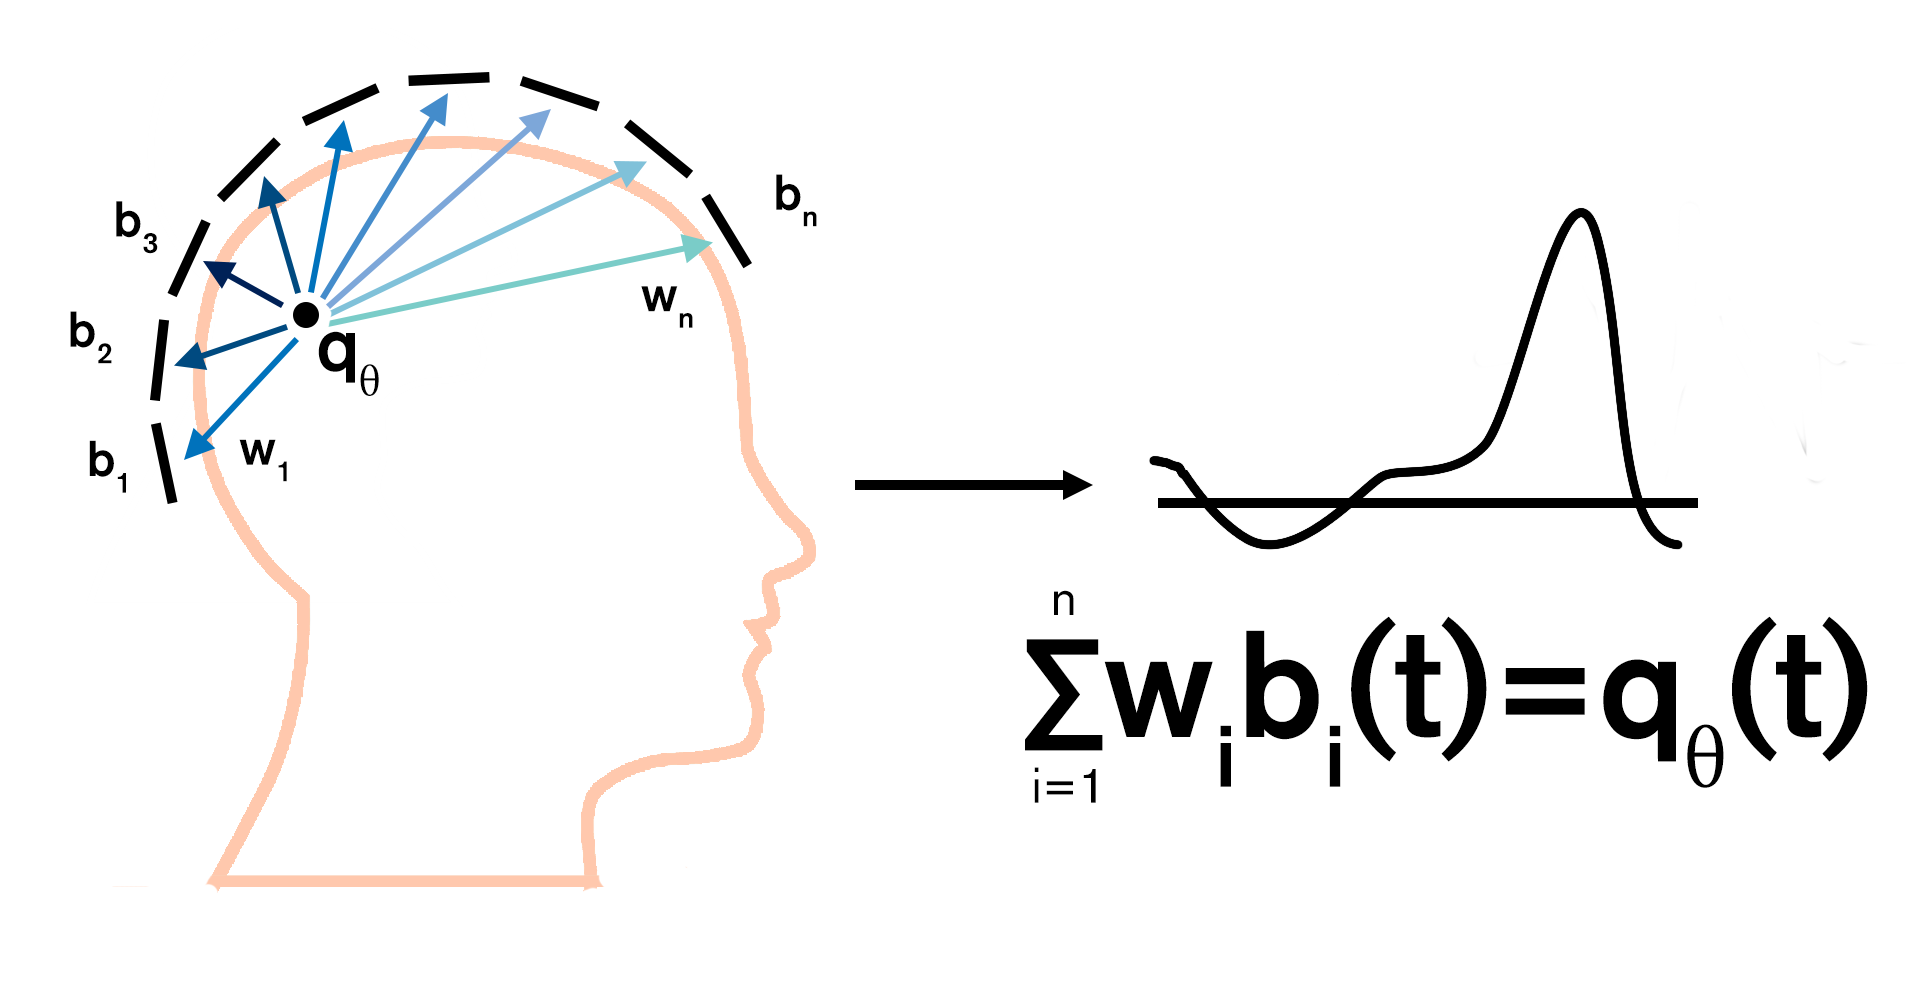
\includegraphics[width=0.8\linewidth]{./images/chapter2/Figure_2.png}
		\caption{A diagram to illustrate the concept of spatial filtering. A source $\mathbf{q_\theta}$ in the brain can be represented as the weighted sum of the extracranial mesurements from an MEG sensor array. The weights of each sensor in this diagram may, for example, scale with distance, represented by the darkness of the arrows representing $w$.\label{figure_2_3}}
	\end{center}
\end{figure}

\subsection{Beamforming}

Beamforming is an alternative approach to spatial filtering which has become a popular alternative to minimum norm estimations, particularly in the imaging of the spatial signature of neural oscillations. First developed for RADAR in World War II,  beamforming was introduced to MEG by \cite{Robinson1992}.

Beamforming starts with the same spatial filter formulation in Equation \ref{eqn_filter_gen}, but instead $\mathbf{w_\theta}$ is based on power minimisation. In particular the output of the beamformer $\hat{q}_\mathbf{\theta}(t)$ is minimised with the constraint that the power at $\mathbf{\theta}$ remains unchanged. If the estimated power is defined as the expectation value of the squared signal 

\begin{equation} \label{eqn_bf_2}
P_{\mathbf\theta} = \big\langle\hat{q}^2_{\mathbf\theta}(t)\big\rangle,
\end{equation}
then the beamformer can be formulated mathematically as 

\begin{equation} \label{eqn_bf_3}
\underset{\mathbf{w_\theta}}{\text{min }}\big(\langle\hat{q}^2_{\mathbf\theta}(t)\rangle\big)\text{, subject to } \mathbf{w}_{\mathbf{\theta}}^T\mathbf{l_\theta} = 1.
\end{equation}
Note that the linear constraint  $\mathbf{w_\theta}^T\mathbf{l_\theta} = 1$ comes from the definition of the lead field model of a unit dipole, meaning power remains at unity. Substituting Equation \ref{eqn_filter_gen} into Equation \ref{eqn_bf_2} gives

\begin{equation}
\begin{aligned}\label{eqn_bf_4}
P_{\mathbf\theta} &= \Big\langle \big(\mathbf{w}^T_{\mathbf\theta}\mathbf{b}(t)\big)\big(\mathbf{w}^T_{\mathbf\theta}\mathbf{b}(t)\big)^T\Big\rangle \\
&= \mathbf{w}^T_{\mathbf\theta}\big{\langle}\mathbf{b}(t)\mathbf{b}(t)^T\big\rangle\mathbf{w}_{\mathbf\theta}\\
&\approx \mathbf{w}^T_{\mathbf\theta}\mathbf{C}\mathbf{w}_{\mathbf\theta},
\end{aligned}
\end{equation}
where $\mathbf{C}$ is the $n \times n$ data covariance matrix of the magnetic field data recorded by the MEG sensor, where the $ij^{\text{th}}$ element is the covariance of the data recorded at channels $i$ and $j$ respectively. In general, if we want to find the extrema of a function, $f(x)$ with the added linear constraint of $g(x)=0$, we can form a composite function called a Lagrangian such that

\begin{equation}
	\mathscr{L}(x,\lambda) = f(x) + \lambda g(x)
\end{equation} where $\lambda$ is a scalar value called a Lagrange multiplier. We can form a Lagrangian describing the power output of the beamformer based on Equation \ref{eqn_bf_3}:

\begin{equation}\label{eqn_bf_8}
\mathscr{L}(\mathbf{w_\theta},\lambda ) = \mathbf{w}^T_{\mathbf\theta}\mathbf{C}\mathbf{w}_{\mathbf\theta} + \lambda (\mathbf{w_\theta}^T\mathbf{l_\theta} - 1).
\end{equation} To satisfy the conditions set by Equation \ref{eqn_bf_3}, we need to solve $\mathbf{\nabla}\mathscr{L}(\mathbf{w_\theta},\lambda )=0$:

\begin{equation}\label{eqn_bf_9}
\frac{\partial \mathscr{L}(\mathbf{w_\theta},\lambda )}{\partial \mathbf{w_\theta}} = 2\mathbf{C}\mathbf{w}_{\mathbf\theta} + \lambda \mathbf{l_\theta} = 0.
\end{equation} Rearranging Equation \ref{eqn_bf_9} gives an expression of $\mathbf{w_\theta}$ in terms of $\lambda$

\begin{equation}\label{eqn_bf_9a}
\mathbf{w_\theta} = -\lambda\mathbf{C}^{-1}\mathbf{l_\theta}/2.
\end{equation} By equating $\mathbf{w_\theta}^T\mathbf{l_\theta} - 1 = 0$ with Equation \ref{eqn_bf_9} it is possible to give an expression for $\lambda$: 

\begin{equation}\label{eqn_bf_10}
\lambda = -2[\mathbf{l}^T_{\mathbf\theta}\mathbf{C}^{-1}\mathbf{l}_{\mathbf\theta}]^{-1},
\end{equation} substituting Equation \ref{eqn_bf_10} into \ref{eqn_bf_9a}, we arrive a a solution for the beamformer weights:

\begin{equation}\label{eqn_weights_bf}
\mathbf{w}_{\mathbf{\theta}_{BF}}^T = \frac{\mathbf{l_\theta}^T\mathbf{C}^{-1}}{\mathbf{l}^T_{\mathbf\theta}\mathbf{C}^{-1}\mathbf{l}_{\mathbf\theta}}.
\end{equation}Note that whilst $\mathbf{C}$ has not been regularised here, it can be Tikhonov regularised like the Gram matrix $\mathbf{G}$. Here, $\mathbf{C}_r = \mathbf{C} + \eta\mathbf{I}$ where $\eta$ is a scalar parameter and $\mathbf{I}$ is an $n\times n$ identity matrix. 

\subsection{Determining source orientation}\label{sec_334}

A core parameter of a successful source reconstruction is the source orientation. Thus far, we have assumed that the orientation of a source was known, but in practice this is not the case. A correct estimation of these angles is important, as along with source location, orientation has an effect on the weighting parameter, $\mathbf{w}$. Whilst it is known that the sources seen in MEG are unlikely to be radial, it could exist at one of many other orientations. There are two popular approaches to finding the optimal orientation, both of which follow the underlying principle that the best orientation to model is the one which gives the maximal SNR for a given location.

\subsubsection{Exhaustive search method} In this method, the orientation is found from an exhaustive search of all possible orientations. However, as we assume radial sources do not contribute to the MEG, the orientation of a dipole is constrained to remain azimuthal to the surface of the brain, determined from the head model derived from the anatomical image of the subject. Consequently, this reduces the complexity and the size of the search. From here multiple dipoles are modelled, all at different angles of $0 \leq \phi \leq \pi$, where $\phi$ is the azimuthal angle. For every orientation of $\phi$ at a given position \textbf{r}, the corresponding weight vectors are calculated and then a search for the maximal SNR is performed  by measuring the pseudo-Z statistic for each orientation. In the case of a beamformer this is calculated by:

\begin{equation}
\text{\sout{Z}}_{\mathbf{r},\phi} = \frac{\mathbf{w}_{\mathbf{r},\phi}^T\mathbf{C}\mathbf{w}_{\mathbf{r},\phi}}{\mathbf{w}_{\mathbf{r},\phi}^T\mathbf{\Sigma}\mathbf{w}_{\mathbf{r},\phi}},
\end{equation} where $\mathbf{\Sigma} = \sigma^2\mathbf{I}$ is the noise covariance matrix, $\sigma^2$ is the uncorrelated noise power at each MEG sensor and $\mathbf{I}$ is an identity matrix. $\phi$ is determined from the maximum value of $\text{\sout{Z}}_{\mathbf{r},\phi}$ and the corresponding column of weights is selected for reconstruction. This method (for arcane reasons in the Nottingham MEG group) is used to determine source orientation. 

\subsubsection{Eigenvalue decomposition}

An alternative method was proposed by \cite{Sekihara2004}. In an eigenvalue orientation determination the objective is to reconstruct a 3-element dipole timecourse for a given location and find the combination of those three timecourses which gives maximal variance. To achieve this the weights for a given location are calculated in three orthogonal orientations, $[\mathbf{w}_{r_i}, \mathbf{w}_{r_j}, \mathbf{w}_{r_k}]$ and three source timecourses are reconstructed to form  $\mathbf{q}_r = [\mathbf{q}_{r_i}, \mathbf{q}_{r_j}, \mathbf{q}_{r_k}]$. Note that the orientations of $i$, $j$ and $k$ are perpendicular to each other, but otherwise arbitrary. To find the maximal variance, the first principal component of $\mathbf{q}_r$ is calculated, to give a solution which is equivalent to the scalar solution.  

\subsection{Depth correction}\label{sub_depthcorrection}

The problem with the weights derived for minimum norm and beamforming in Equations \ref{eqn_weights_mn} \& \ref{eqn_weights_bf} is that they have a tendency to mislocalise sources. For the minimum norm spatial filter, it tends to bias sources nearer the sensors (i.e it pulls sources towards the outside of the brain \citep{Fuchs1999,Lin2006}) due to attenuation of the lead fields for deeper sources. This has led to the development of a series of "weighted minimum norm" solutions which come in many varieties \citep{Fuchs1999,Dale2000,Pascual-Marqui2002,Lin2006} but all share the same goal of implementing a depth correction step into the source reconstruction. One popular variant, dynamic Statistical Parametric Mapping (dSPM) \citep{Dale2000} attempts to normalise the minimum norm weights by their own norm, ensuring an even noise distribution across the entirety of the brain. 

\begin{equation} \label{eqn_weights_dspm}
	\begin{aligned}
		\mathbf{w}^T_{\mathbf{\theta}_{dSPM}} &= \frac{\mathbf{l}^T_\mathbf{\theta}\mathbf{G}^{-1}}{\big\|\mathbf{w}_{\mathbf{\theta}_{MN}}^T\big\|} \\
		& = \frac{\mathbf{l}^T_\mathbf{\theta}\mathbf{G}^{-1}}{\sqrt{\mathbf{l}^T_\mathbf{\theta}\mathbf{G}^{-2}\mathbf{l}_\mathbf{\theta}}}.
	\end{aligned}
\end{equation} For beamformers the bias is toward the centre of the brain. This occurs due to norm of the lead fields falling towards the centre, which in turn increases the norm of the beamformer weights for deeper sources and increases their variance. Again, this is compensated for by scaling the beamformer weights by their own norm: 

\begin{equation} \label{eqn_weights_z_1}
	\big\|\mathbf{w}_{\mathbf{\theta}_{BF}}\big\| = \frac{\sqrt{\mathbf{l}^T_\mathbf{\theta}\mathbf{C}^{-2}\mathbf{l}_\mathbf{\theta}}}{\mathbf{l}^T_\mathbf{\theta}\mathbf{C}^{-1}\mathbf{l}_\mathbf{\theta}}.
\end{equation} Dividing Equation \ref{eqn_weights_bf} by \ref{eqn_weights_z_1} gives the depth corrected beamformer weights:

\begin{equation} \label{eqn_weights_z_2}
\mathbf{w}^T_{\mathbf{\theta}_{\text{\sout{Z}}}} = \frac{\mathbf{l}^T_\mathbf{\theta}\mathbf{C}^{-1}}{\sqrt{\mathbf{l}^T_\mathbf{\theta}\mathbf{C}^{-2}\mathbf{l}_\mathbf{\theta}}}.
\end{equation} Here the subscript \sout{Z} denotes that the depth corrected bemformer weights do not produce a current dipole with units Am, but instead a pseudo-Z statistic. Note there is a direct equivalence between equations \ref{eqn_weights_dspm} and \ref{eqn_weights_z_2} \citep{Mosher2003}. The difference between the two reconstruction methods boils down to one being data driven (the data covariance in beamforming) and one being based on a model (the inner product of the modelled lead fields in dSPM). In exceptional circumstances it is possible for the two methods to give identical results. For example, if a unit current dipole existed at every voxel in the brain then $\mathbf{C} = \mathbf{G} $.  

\subsection{Beamformer Noise Rejection}

One of the key features of the beamformer (and arguably one of its advantages) is its ability to efficiently suppress sources of interference \citep{Sekihara2001,Sekihara2006,Brookes2008}. At a basic level, the spatial topography of interference does not resemble the spatial topography of a neural source.  The minimisation term in Equations \ref{eqn_bf_3} acts to minimise all signals other than those exhibiting a specific source pattern, $\mathbf{l_\theta}$. This means that the artefacts with spatial topographies orthogonal to $\mathbf{l_\theta}$ can be supressed significantly. This is particularly useful for sources of interference such as eye blinks, magnetomyographic (muscular), or magnetocardiographic interference, as these sources (whilst not in the brain) are not far enough away to be effectively regressed out by the MEG reference gradiometers (see Section \ref{sec_1_inteference}). In these situations, using a beamformer to automatically reject these is an attractive feature. 

Figure \ref{fig_bf_reject} shows work by Eleanor Barratt \citep{ONeill2015b} which demonstrates the effectiveness of the beamformer at removing the electrocardiogram from experimental data. Here, 600 s of resting state MEG data have been recorded from a single subject using our MEG system following the procedures laid out Section \ref{sec_data_acq}. In addition, the subject’s electrocardiogram (ECG) has been recorded concurrently. The magnetic fields generated by the heart are well known to affect MEG data and here the effect of this on sensor space and source space signals has been calculated. The four plots in Figure \ref{fig_bf_reject} show correlation between the ECG and MEG data, plot as a function of frequency. The pink lines show correlation at the sensor level whereas the blue lines show correlation at the source level after reconstruction, via beamforming, at the locations shown by the red markers. The separate plots show the four different locations. Sensor space analysis was undertaken at the 5 sensors corresponding to the largest absolute elements of the forward vectors from the chosen source space locations, with results averaged over sensors. This example shows clearly the effectiveness of beamforming as an interference rejection method: frequency filtered MEG data correlate relatively highly at the sensor level with the (equivalently filtered) ECG. This is particularly true in the low (delta and theta) frequency bands, where, correlation coefficients are as high as 0.6. However when moving into source space, these correlation coefficients are reduced to < 0.1 across all frequency bands and locations studied. This interference rejection is of significant utility; if common mode signals are allowed to interfere with MEG signals from separate locations, then artefactual connectivity will necessarily result if the connectivity analysis does not account for zero-phase relations. By reducing this interference, source space estimates of connectivity are likely to be more accurate reflections of true coupling between regions. 

\begin{figure}[h!]
	\begin{centering}
		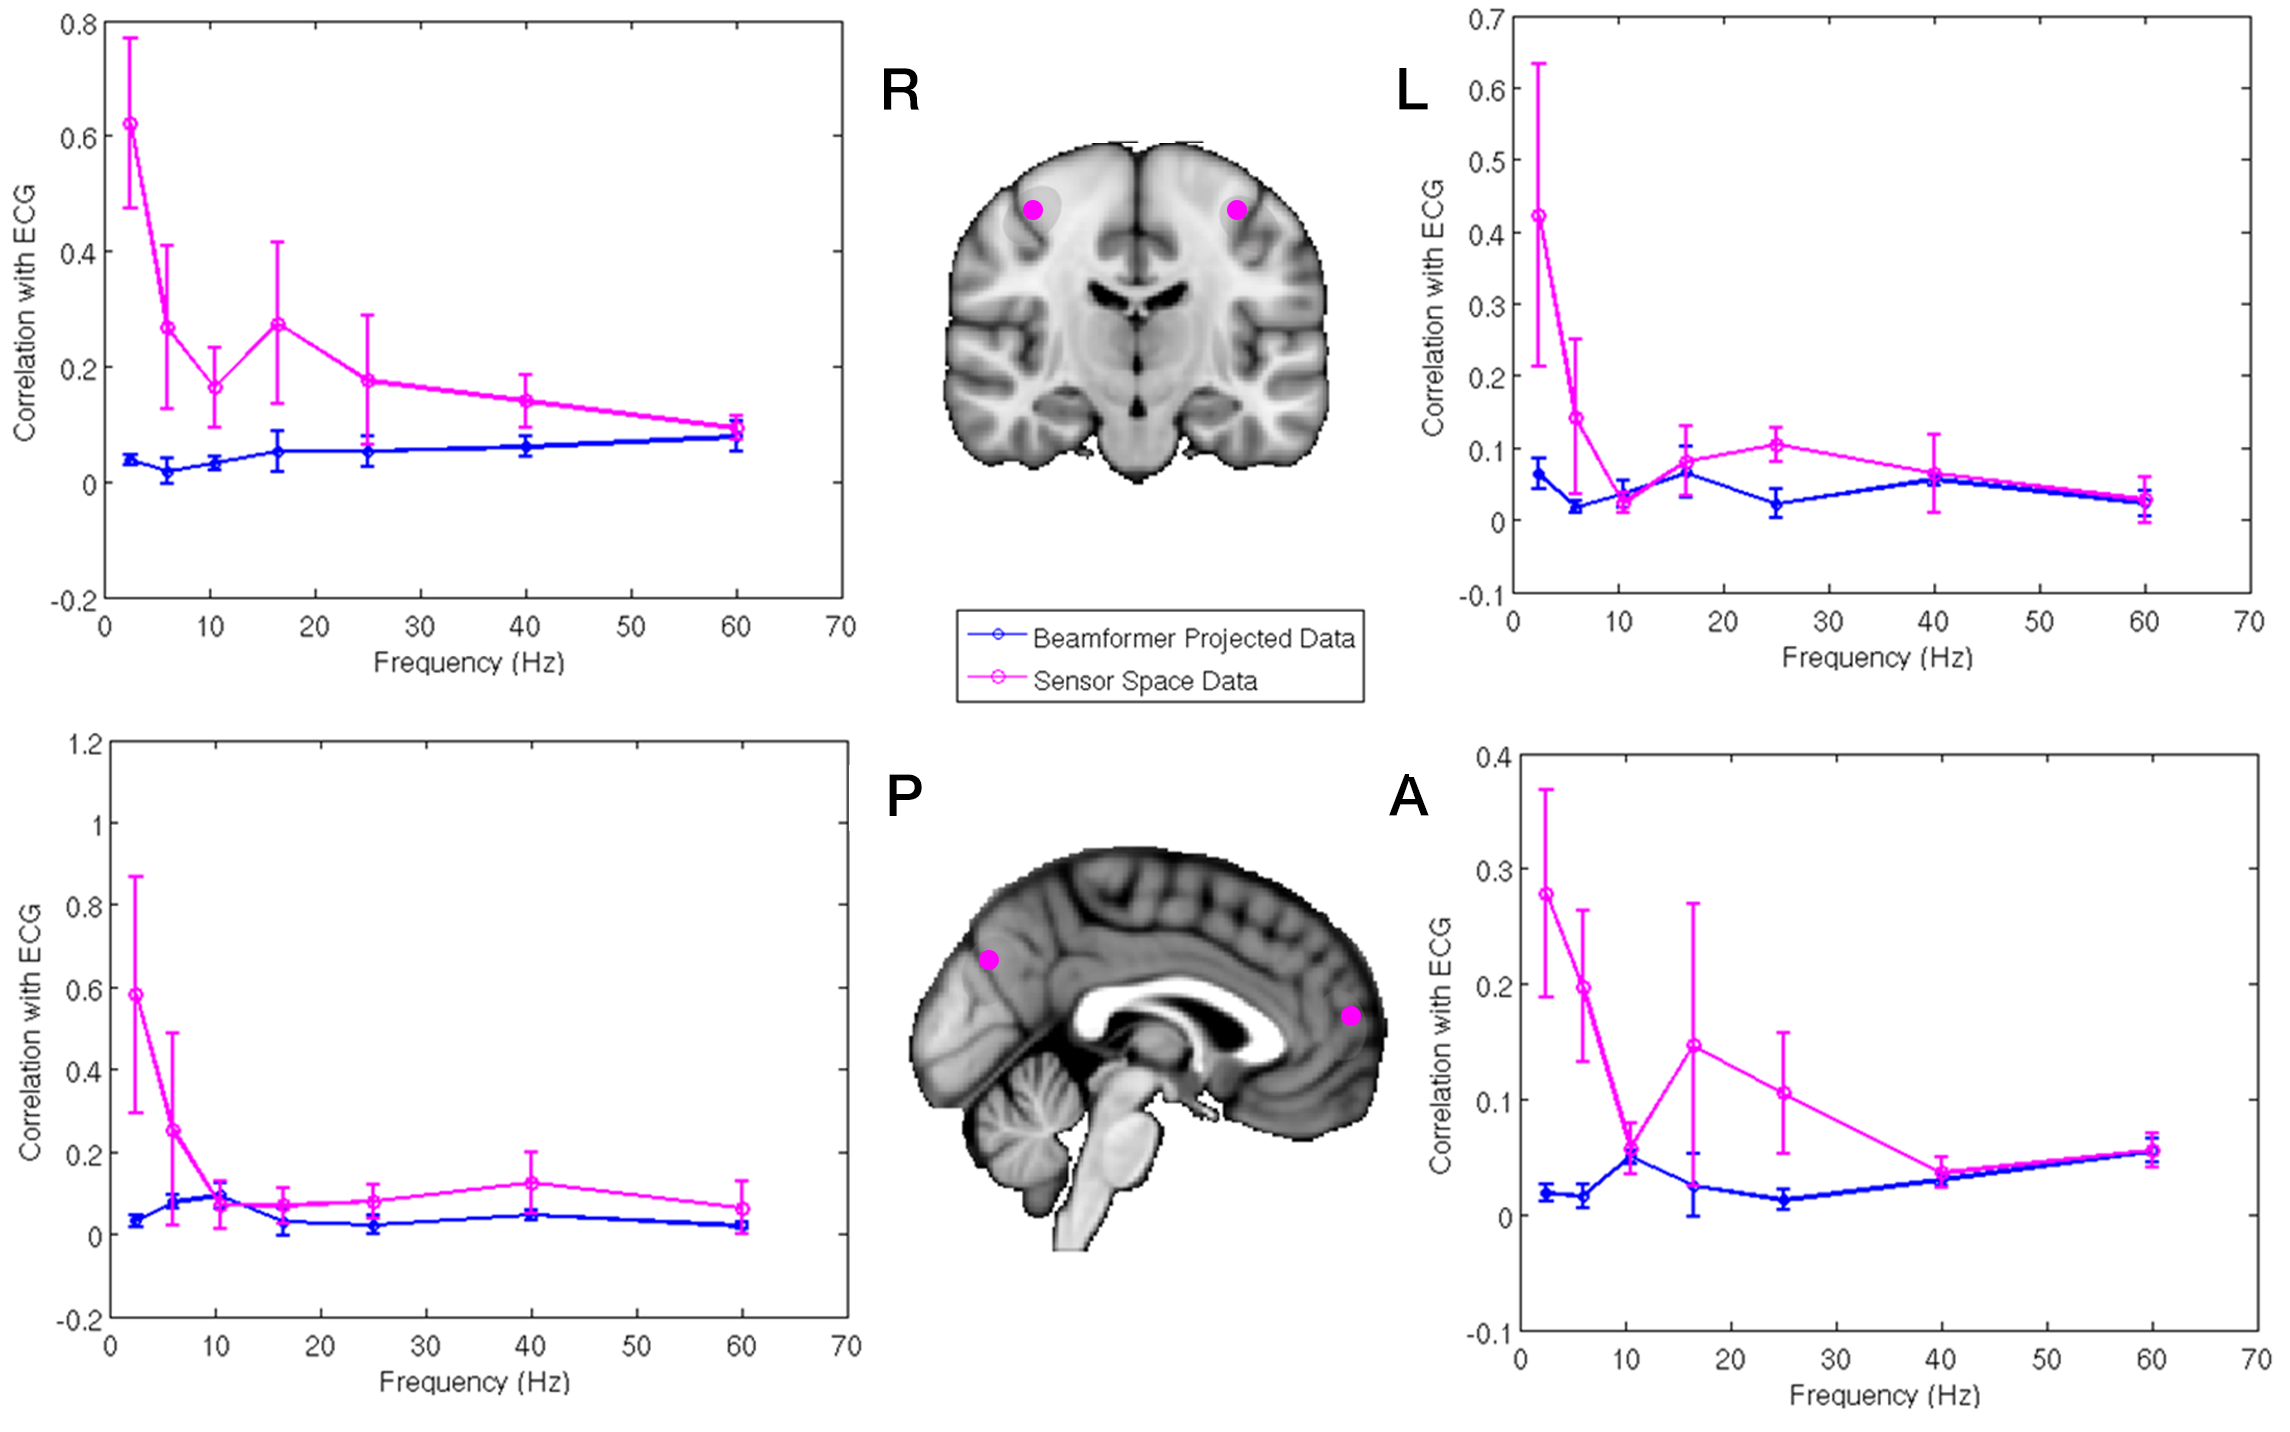
\includegraphics[width=\textwidth]{./images/chapter2/beamformer_reject.png}
		\caption{An example of interference rejection by beamforming. The four plots show correlation between the measured electrocardiogram and MEG data. The pink lines show correlation at the sensor level whereas the blue lines show correlation at the source level. The separate plots show different brain locations – the source space analysis was undertaken at brain locations indicated by the red markers. The sensor space analysis was undertaken at the 5 nearest sensors with the largest magnitude forward vectors  for a ROI. Note the excellent reduction in cardiac interference afforded by beamforming. Figure adapted from work by Eleanor Barratt \citep{ONeill2015b}}
		\label{fig_bf_reject}
	\end{centering}
\end{figure}

\clearpage
\section{Comparing inverse solutions for functional connectivity mapping}\label{sec_bf_v_mn}

Both beamforming and minimum norm solutions have been used extensively in functional connectivity analysis (cf. \citealp{Brookes2011,Luckhoo2012,Baker2014,ONeill2015A} for beamforming examples and \citealp{dePasquale2010,Pavla2010,Marzetti2013,Wens2014a} for studies using MNE-type methods) to overcome the issues raised in the introduction to this chapter and due to the gain in SNR in source space compared to sensor space. However it is unclear whether one inverse solution is better suited to the challenges functional connectivity analysis presents. There are many differences in the behaviour of both kind of inverse solutions, however to describe them all could be a thesis in itself, so only a few examples here are given. Beamforming can in exceptional cases confound connectivity analysis; for example, multiple studies have shown that beamforming fails to reconstruct bilateral auditory steady state evoked sources \citep{Dalal2006,Brookes2007,Popescu2008,Diwakar2011} due to the high correlation between signals generated by sources in opposite hemispheres. Such a failure in reconstruction would clearly lead to artefactual task induced auditory connectivity estimates, and may also impact upon resting state investigations. In such cases minimum norm variants would prove advantageous since they are able to reconstruct correlated sources. However that is not to say minimum norm estimations are without  faults. As minimum norm attempts to explain the complete set of measured fields, any remnant interference not eliminated will be introduced at a source level. In addition insufficent modelling of the Gram matrix (by not calculating the lead fields over enough of the brain volume) can lead into complete mislocalisation of sources.  These examples are just some of many differences between to two categories of inverse solutions, but as mentioned in the Section \ref{sub_depthcorrection}, they are mathematically equivalent to each other when depth corrected, save for the difference between \textbf{C} and \textbf{G}. Reviews and comparisons of inverse methods have been compared in the past \citep{Mosher2003,Scoffelen2009,Hauk2011}, but direct comparisons of these methods in the context of ability to aid or impede functional connectivity estimates have not been conducted. Here, we investigate whether the selection of inverse solution has a profound effect on the results of previously established, static functional connectivity analysis methods \citep{Brookes2011,Luckhoo2012,Hall2013} by simultaneously analysing functional data using both dSPM and weight normalised beamforming, selected for their mathematical equivalence.

\subsection{Methods}
\subsubsection{Data Acquisition}
All data were collected using a CTF MEG system as described in Section \ref{sec_data_acq}. Experiments were approved by the University of Nottingham Medical School Ethics Committee. \textit{(Note: the experiments themselves were performed by other researchers within the SPMIC and acquired from the archives, but the analysis described was conducted by GCO.)} Data from two studies were employed. 

\begin{itemize}
\item \textbf{Study 1} -- \textit{Resting State Study:} 9 subjects were asked to lie in the scanner for 1800 seconds. 600 seconds with the participants eyes open, 600 with their eyes closed and 600 whilst watching a movie. The three recordings were done consecutively, but as individual datasets. To allow for the removal of SQUID reset artefacts, all scans were split into 10 second blocks. 
\item \textbf{Study 2} -- \textit{N-Back Study:} 8 subjects were shown a series of letters, one every 2 seconds. Subjects were asked to respond (via a button press with their right index finger) when the present letter matched that presented N letters previously. 5 conditions were assessed; 0-back (respond when an X is on display), 1-back, 2-back, 3-back and rest. 1800 seconds of data were recorded in one acquisition.
\end{itemize}

\subsubsection{Data Processing}
All data were subject to a visual inspection for artefacts from SQUID resets or for strong interference (magnetomyographic, magnetocardiographic and ocular effects), and any trials which contained excessive interference were removed. All data were then band pass filtered in the $\beta$-band (13-30 Hz). The covariance matrix $\mathbf{C}$ was generated using these filtered-data across all time. The regularisation parameter $\mu$ was calculated for $\mathbf{G}$ so that it would equate the condition numbers for $\mathbf{C}$ and $\mathbf{G}$. Timecourses were then constructed using both beamformer and dSPM solutions (weights were based on Equations \ref{eqn_weights_dspm} and \ref{eqn_weights_z_2}), at the vertices of an isotropic 8mm grid spanning the entire brain. In all cases a multiple local sphere volume conductor head model \citep{Huang1999} was employed and the forward solution was based on a dipole model \citep{Sarvas1987}. Source orientation was defined as that generating maximum projected SNR for each voxel. Amplitude envelope timecourses were computed \textit{via} Hilbert Transform of the projected data (see Section \ref{sec_3_hilbert} for a full mathematical description) and downsampled to an effective 1 second time resolution, which maximises the SNR of the envelopes \citep{Luckhoo2012}. The resultant timecourses were then coregistered to a standard brain space using the FMRIB Linear Image Registration Tool (FLIRT) in FSL \citep{Jenkinson2012}.   

\subsubsection{Deriving Functional Networks with Temporal ICA} To reveal the functional networks within the resting state data, we used previously published methods \citep{Brookes2011,Luckhoo2012,Hall2013} based on temporal Independent Component Analysis (tICA). ICA is a multivariate blind source separation technique, which collapses the several thousand amplitude envelopes generated across many voxels in the brain into a small set of temporally independent components. A graphical representation of ICA can be found in Figure \ref{fig_bf_mn_ic}, and a mathematical description follows. If we have an array  of measurements in a matrix \textbf{X}, which is of dimensions $n\times s$, $n$ representing the number of signals and $s$ the number of samples, we say that our measurements can be explained as a linear superposition of a set of temporally independent components (ICs). Mathematically:

\begin{equation}
\mathbf{X} = \mathbf{AS}+\mathbf{\epsilon},\label{eqn_ica}
\end{equation} where the rows of $\mathbf{S}$ are linearly independent components and the columns of \textbf{A} represent the mixing coefficients of each IC to every measurement; that is to say, the linear sum of voxels which a component is generated from. The matrix $\mathbf{\epsilon}$ represents the unexplained data. In functional connectivity we assume that each functional network is characterised by an independent timecourse of neural activity (i.e. an independent component) and the network topography can be represented with the corresponding column of \textbf{A}. ICA estimates the unmixing matrix, \textbf{W}, which gives the total contribution of each timecourse to each IC. 
\begin{equation}
\mathbf{S} = \mathbf{WX}.
\end{equation}

\begin{figure}[h!]
	\begin{centering}
		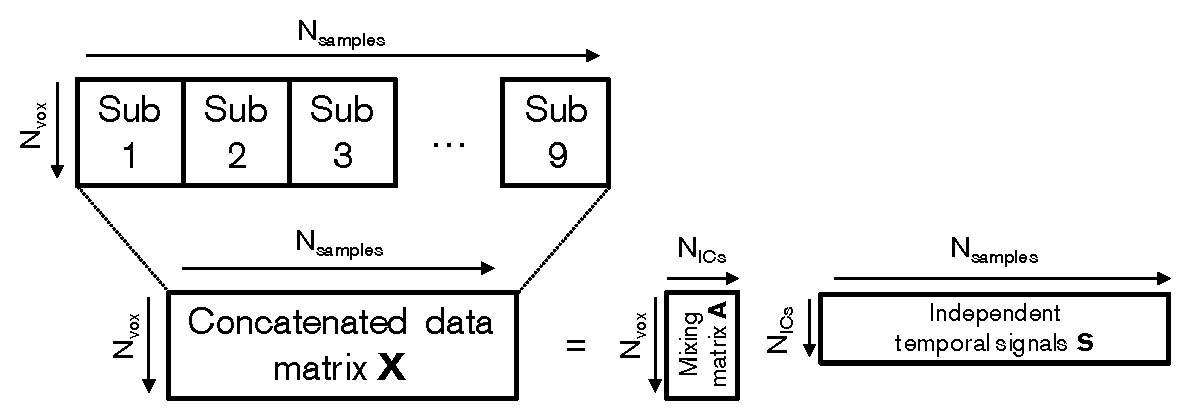
\includegraphics[width=0.9\textwidth]{./images/chapter2/ica.pdf}
		\caption{A schematic representation of ICA.}
		\label{fig_bf_mn_ic}
	\end{centering}
\end{figure}

To prepare our downsampled envelope data for ICA, the coregistered subject timecourses were mean corrected and normalised by dividing by global standard deviation of all timecourses for that subject. Dividing all timecourses by a single value reduces the variance across subjects, but preserves the variance across voxels within a single subject;  allowing for a better assessment of the spatial signatures of the resultant independent components \citep{Hall2013}. The timecourses were reshaped into a $n\times ft$ array, where $n$ is the number of timecourses, $f$ is the sample rate (1 Hz) and $t$ is the length of the recording in seconds. Individual arrays were concatenated across time to form the measurement matrix \textbf{X}. Data were pre-whitened using principal component reduction, with the first $N_{\text{ICs}}+5$ principle components kept, where $N_{\text{ICs}}$ represents the target number of independent components required. Temporal ICA was then applied with $N_{\text{ICs}}=20$ independent components  generated for beamformer reconstructed data and 25 for minimum norm data using the FastICA algorithm \citep{Hyvarinen1999}, with a deflation decomposition approach utilised. 


The resultant temporal ICs from both inverse solutions were then compared to each other to find similarities. Every beamformer IC was temporally correlated using a Pearson correlation to every minimum norm IC and then ordered from highest correlation to lowest. The best match for each beamformer IC was kept and then the spatial correlations (respective columns of \textbf{A}) were correlated. After this the relevant columns of \textbf{A} were reshaped back into 3D and presented.   

\subsection{Results}

Figure \ref{fig_bf_mn_3} shows the results of the temporal correlation between the independent components generated for both beamformer and minimum norm methods. The first column of the matrix shows the corresponding IC number from the beamformer ICs, the second shows the minimum norm counterpart which has the largest temporal correlation, the third shows the second highest correlation and so on. The correlation matrix shows that in most cases there is a high correlation between a beamformer IC and one other MNE IC, with occasionally two MNE ICs shown to be similar. The correlation matrix has also been sorted to show the strongest correlating pair at the top, with progressively poorer matches placed toward the bottom. The best match corresponds to a temporal correlation coefficient of $r_t = 0.65$. The correlations between best matches quickly reduce from 0.65 to less than 0.3 after 10 components. Figure \ref{fig_bf_mn_4} shows the spatial profiles of the functional networks derived from tICA with the highest $r_t$ values. These networks represent the frontoparietal, motor and visual resting state networks. Results show clear similarity in terms of spatial topography, which is reflected in their high spatial correlations ($r_s$). This implies that whilst different inverse methods may offer specific advantages, resulting network patterns can be highly similar.   

Figure \ref{fig_bf_mn_5} shows the results of the N-Back study analysis. Panel A shows frontoparietal networks extracted using both beamforming and minimum norm. These were paired together using the same methods as depicted in Figure \ref{fig_bf_mn_3}. The networks have a temporal correlation of $r_t = 0.61$ and a spatial correlation of $r_s = 0.75$. A 'sharper' definition is notable in the N-back frontoparietal networks than their resting state equivalents. This is likely due to fewer data coregistration errors in the dataset (8 sets of errors in N-back, compared to 27 in the resting state data). Panels B and C show the mean signal and variance of the voxel timecourses within each network using both inverse solutions. Previous work \citep{Brookes2012a} has shown that, on average, there are distinct temporal properties of networks which are dependent on the difficulty of the N-back task. In particular, it has been show there is a monotropic reduction in the reconstructed signal power in the frontoparietal network when the task difficulty, \textit{N} (the number of prior stimuli a subject needs to remember), increases. The results here agree with this and most importantly both inverse solutions show similar behaviour to each other.

%\begin{figure}
%	\begin{centering}
%		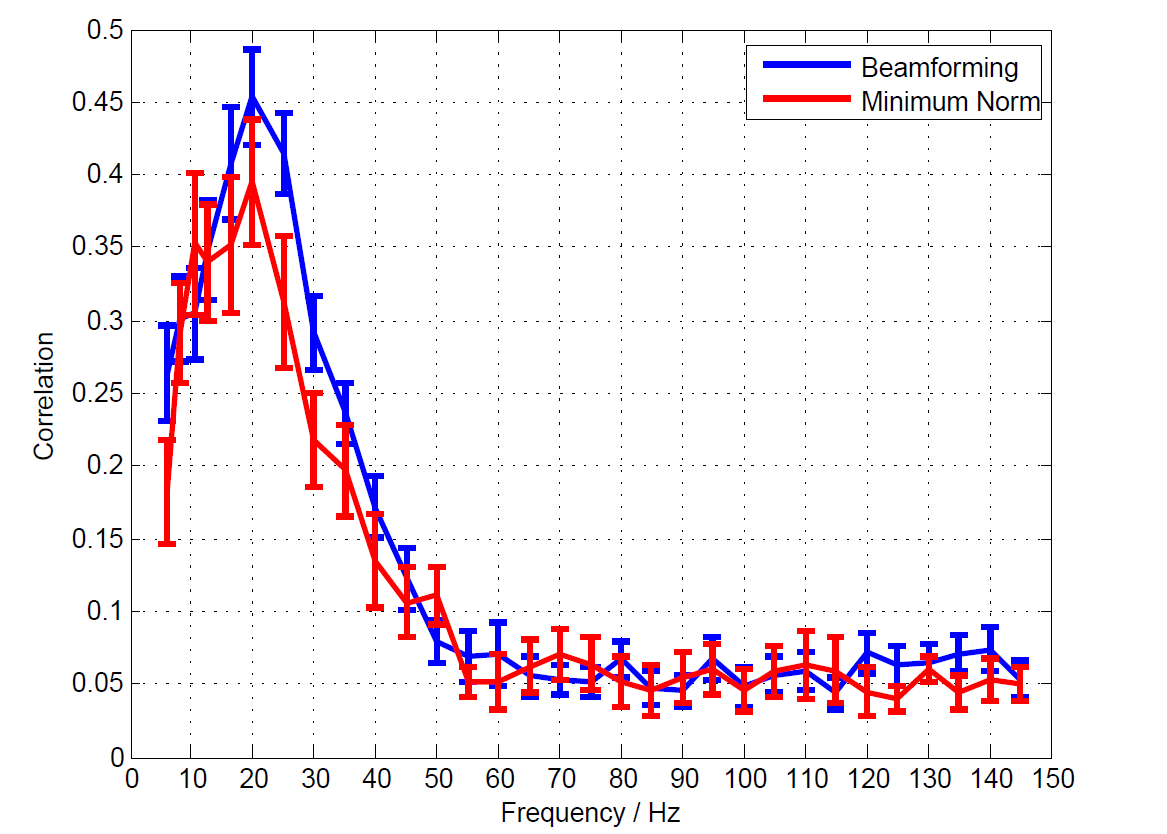
\includegraphics[width=0.75\textwidth]{./images/chapter2/Spectal_Bands.png}
%		\caption{Temporal correlation
%				between envelope signals from left and right motor cortex, plotted as a function
%				of frequency. Result shows the average $\pm$ standard error across subjects. Both
%				inverse algorithms show peak correlation in the $\beta$ (13-30 Hz) band.}
%		\label{fig_bf_mn_2}
%	\end{centering}
%\end{figure}

\begin{figure}[h!]
	\begin{centering}
		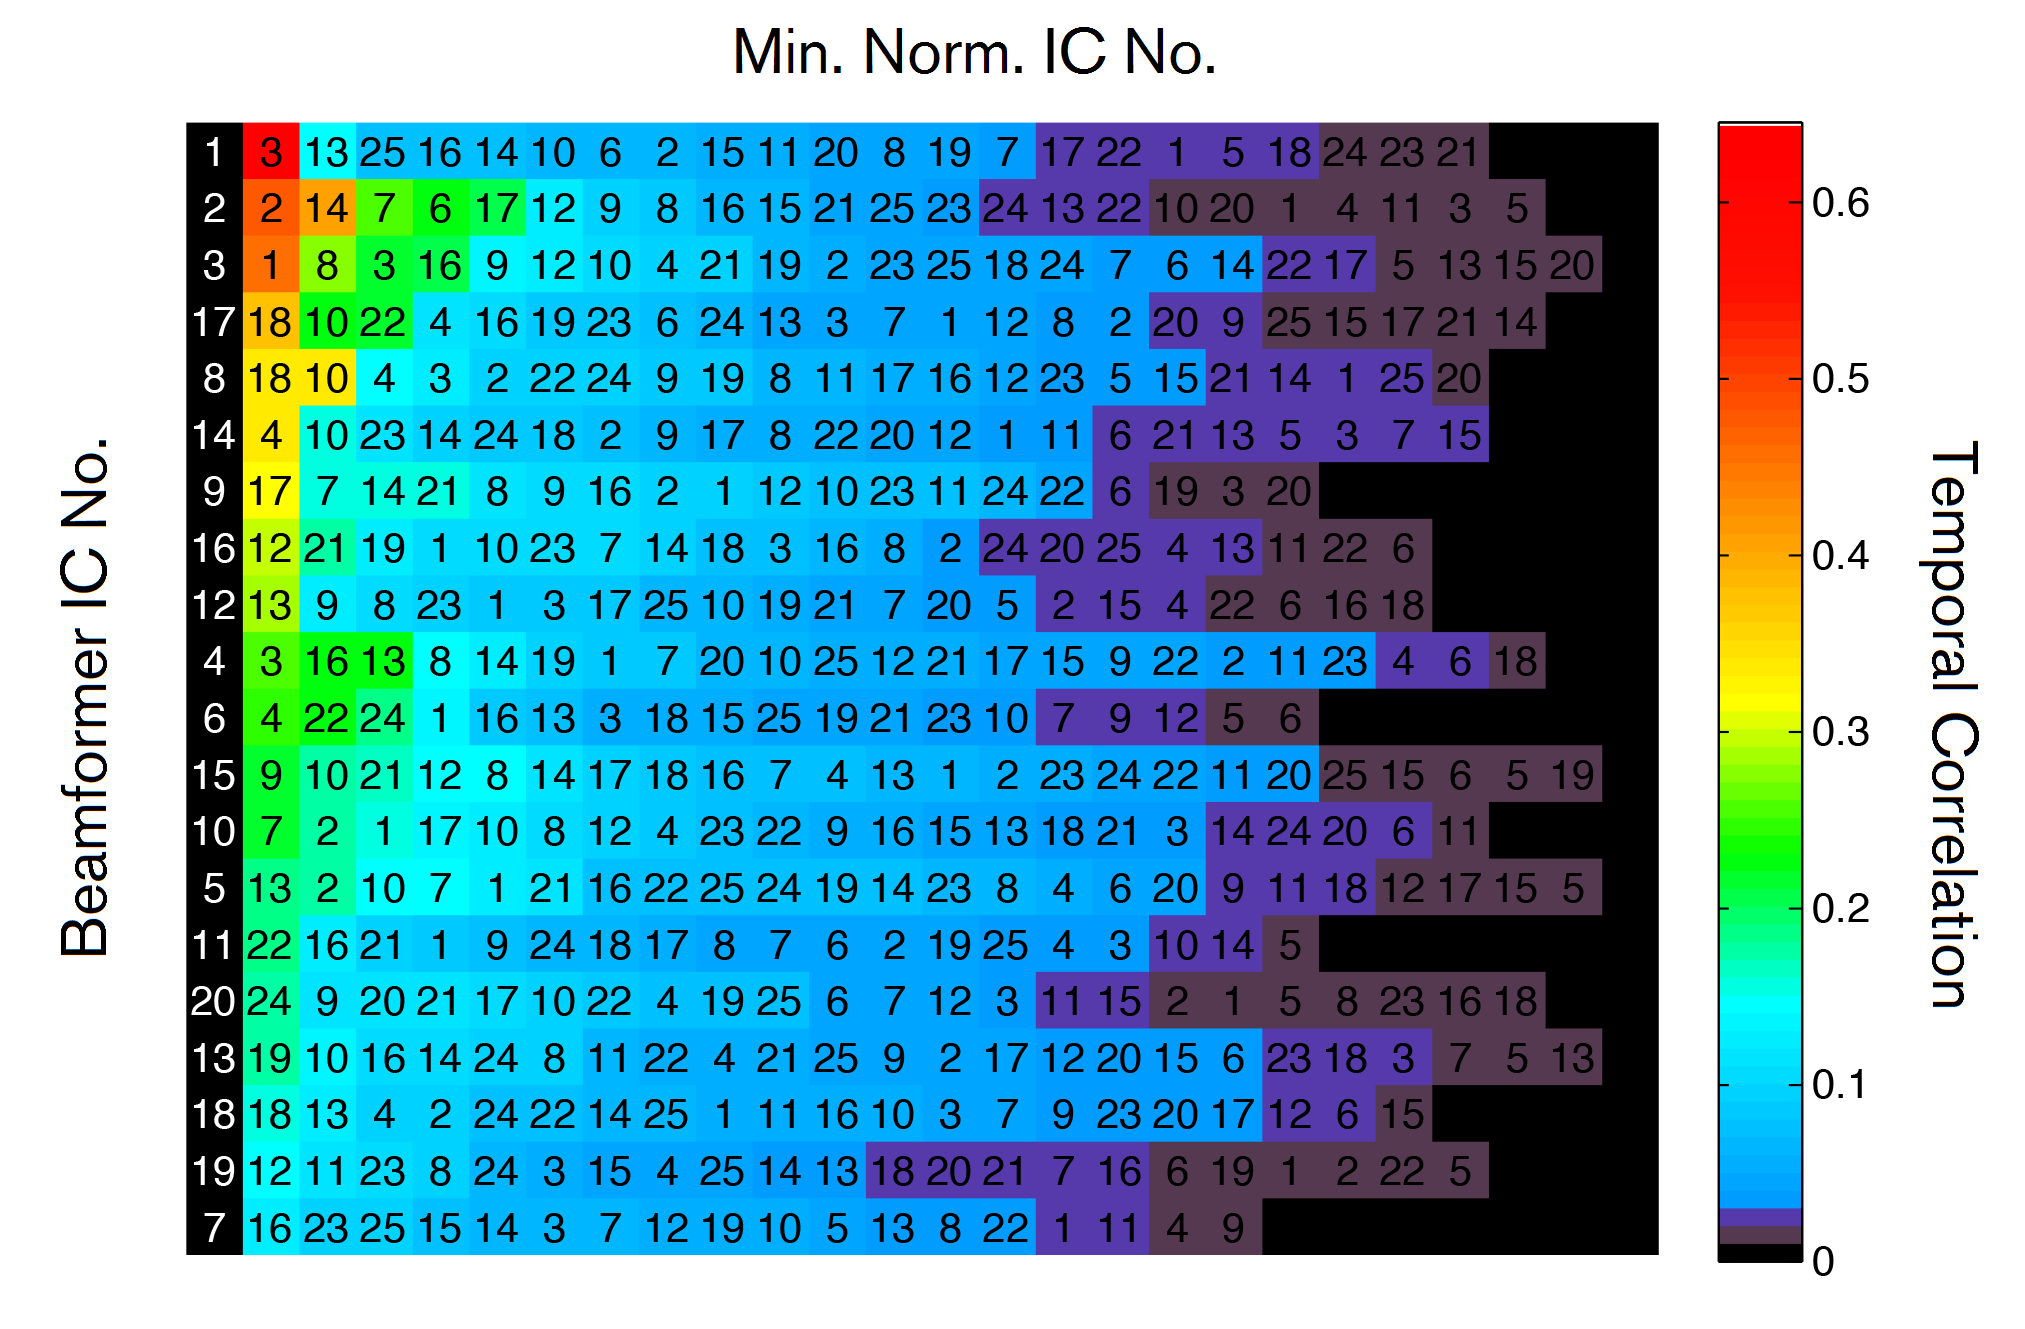
\includegraphics[width=0.9\textwidth]{./images/chapter2/CCmat_2sort.png}
		\caption{Results from the resting state data. The temporal correlation matrix of the 20 beamfoming ICs (leftmost black column) and 25 corresponding MN ICs, (multicoloured rows) with their respective correlations colour coded. They have been sorted such that the strongest correlations are on the left and  best matched pairs are at the top.}
		\label{fig_bf_mn_3}
	\end{centering}
\end{figure}


\begin{figure}[h!]
	\begin{centering}
		\includegraphics[width=\textwidth]{./images/chapter2/fig_03.png}
		\caption{Spatial distributions of temporally matched functional networks, derived from both beamformer and MNE reconstructed resting state MEG data. Spatial topographies of 3 networks (Visual, Motor and Fronto-Parietal) are shown, based on the columns of the mixing matrix \textbf{A} in Equation \ref{eqn_ica}. Networks were thresholded at an arbitrary level for clarity.  Note the similarity across the two inverse methods.}\label{fig_bf_mn_4}
		\end{centering}
	\end{figure}

\begin{figure}[h!]
	\begin{centering}
		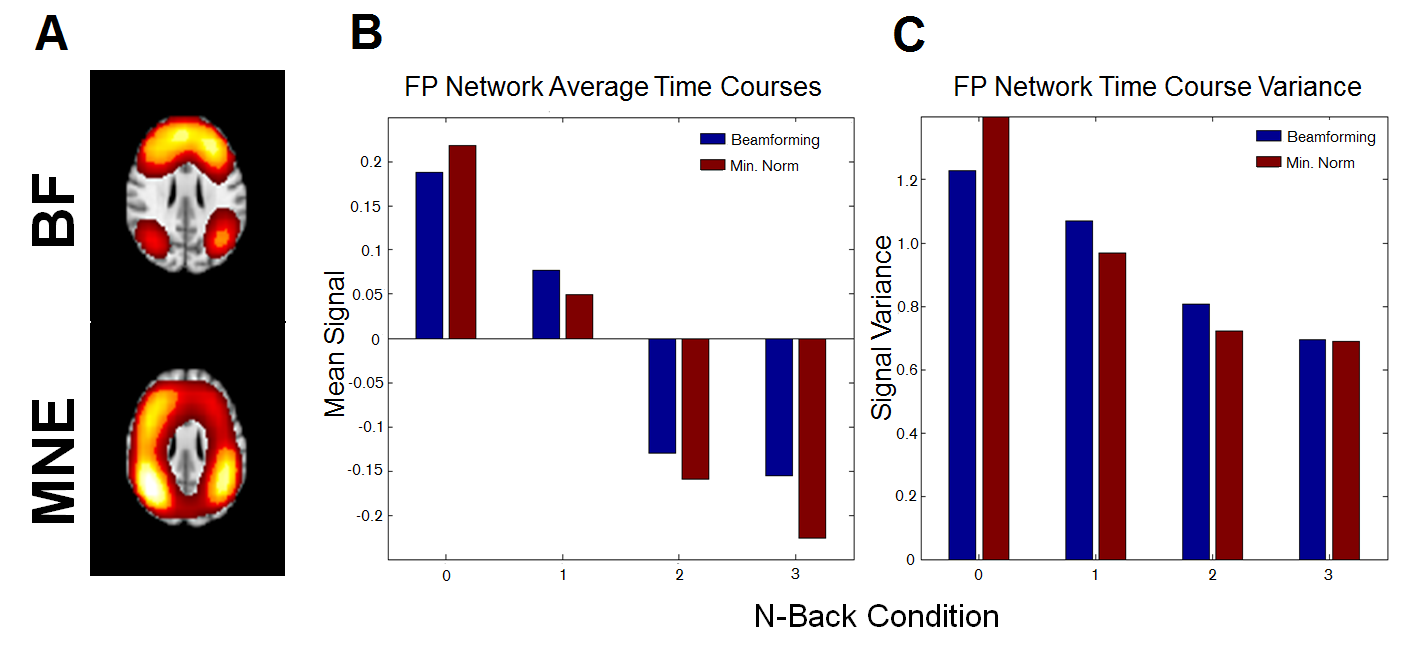
\includegraphics[width=\textwidth]{./images/chapter2/Nback.png}
		\caption{Results from the N-Back study. A) Fronto-parietal Network, extracted using ICA applied to the N-Back data. B-C) The mean signal and signal variance of the IC timecourses corresponding to the fronto-parietal network. Bar charts show the case for beamformer (blue) and minimum norm (red) solutions.
			}\label{fig_bf_mn_5}
		\end{centering}
	\end{figure}
	
	\clearpage	
\subsection{Discussion}

In this investigation, we aimed to assess the effectiveness of two inverse solutions (beamformers, and minimum norm) with regards to functional connectivity mapping. The question posed in the introduction was: can both these methods, even though their underlying assumptions are fundamentally different, produce similar connectivity results in time, space, and the estimated network response to a task? Focusing first in the time domain, we selected an arbitrary threshold of $r_t > 0.3$ to define meaningful correlation between beamformer and minimum norm derived components. Using this criterion, it was found that many beamforming ICs would strongly correlate to (in most cases) just one minimum norm IC. The strongest correlation in the resting state data (top-left element in red in Figure \ref{fig_bf_mn_3}) had a correlation of  $r_t = 0.65$, this implies that both inverse methods share significant temporal characteristics when SNR is adequate. These temporal similarities appear to be robust across studies as the networks could be replicated with both solutions in the N-Back task. In addition these temporal similarities mean that the results of the N-Back study in Figure \ref{fig_bf_mn_5}B and C are similar, with both solutions showing the same isotropic decline variance in the Frontoparietal network when the task increases in difficulty. 

When assessing the spatial attributes of the two methods the similarities continue. The spatial correlations of the reconstructed electrophysiological networks are largely higher than their temporal counterparts. However this may be due to the lower dimensionality of the data in the spatial domain (which corresponds to approximately the number of sensors in a MEG system, in this case it was $\sim$275). Qualitatively, it is not difficult to see that whilst there are some notable differences in the network maps, the general topographies are similar.

Whilst there are clear similarities shown, there are some differences in the network topographies between these two solutions. As the depth scaled equations for both weights (Equations \ref{eqn_weights_dspm} and \ref{eqn_weights_z_2}) differ in only which matrix ($\mathbf{C}$ and $\mathbf{G}$) is in between the lead fields, it is imperative to understand what both are doing. $\mathbf{C}$ being data driven has been shown to make reconstruction more sensitive in areas where activity is more pronounced and less so to brain regions with low SNR \citep{VanVeen1997,Gross2001,Barnes2003}, which makes it ideal at reconstructing oscillatory sources over small regions of brain volumes by accentuating oscillations over a small spatial region. The gram matrix $\mathbf{G}$ however, is a model based upon the geometry of the brain and its position in the MEG system, which gives a similar sensitivity profile around the cortex, giving its reconstructions a 'smudged' characteristic.

That question is, given the similarity of the results, which reconstruction method do we select? Here, we have selected beamformers for a number of reasons. It could be argued that the correlated source suppression will be a hindrance when assessing functional connections, but in practice it will only happen when the correlation between sources is 0.7 or higher \citep{VanVeen1997} or highly correlated for over 40\% of the window which covariance is estimated \citep{Hadjipapas2005}; in practice this is unlikely other than in special cases (such as binaural steady state experiments) or if covariance is assessed over short windows. Secondly, whilst minimum norm is better at reconstructing large regions of evoked activity \citep{Ou2009}, we are intending to look at oscillatory power signatures at smaller spatial scales of connectivity, of which the power estimation of beamforming is better suited \citep{Jensen2010}. This is because unlike minimum norm, it does not try to localise sources based on observations, but rather estimates power at a selected ROI. Also there is the issue of the lack of interference rejection in minimum norm. Whilst you could regress out interference with ICA de-noising methods \citep{Mantini2007}, the automatic rejection of interference with beamforming is an attractive feature. Likewise, not having to make an \textit{a-priori} selection of the number of sources to model makes it particularly flexible for assessment of connectivity on multiple spatial scales; which is useful in the context of the work presented in this thesis, which operates at a single voxel level up to large volumes of brain space. As a final note the MEG laboratory here in Nottingham has gained extensive experience with beamformers over the past decade \citep{Brookes2005,Brookes2007,Brookes2008,Zumer2010,Stevenson2011,Brookes2011a} and so we are in a better position to use them.
\clearpage

\section*{Summary}

In this second theory chapter, we have explained the necessary steps to successfully localise MEG sources, which allows us to circumvent the confounds of sensor level functional connectivity analysis. In reconstructing data back into source space, we allow ourselves to gain a deeper understanding of where functional connections may occur. In the next chapter we introduce methods of functional connectivity analysis which take advantage of the spatial specificity our MEG data now possesses, and crucially the high temporal resolution to image dynamic functional connections.  